\documentclass[10pt]{article}

% =============================================================================
% DATOS GENERALES DEL TRABAJO
% =============================================================================
\newcommand{\materia}{Procesamiento de Señales e Imágenes Biomédicas}
\newcommand{\institucion}{Instituto Tecnológico de Buenos Aires}
\newcommand{\numeroTP}{}
\newcommand{\nombreTP}{Trabajo Práctico final}
\newcommand{\anioTP}{2026}

% =============================================================================
% FORMATO EXIGIDO POR LA CÁTEDRA
% =============================================================================
\textheight=21cm
\textwidth=15cm
\topmargin=-0.5cm
\oddsidemargin=1cm
\evensidemargin=1cm
\parindent=0mm

% =============================================================================
% PAQUETES
% =============================================================================

% Codificación e idioma
\usepackage[utf8]{inputenc}
\usepackage[T1]{fontenc}
\usepackage[spanish,es-tabla]{babel}

% Matemática y unidades
\usepackage{amsmath,amssymb}
\usepackage{siunitx}
\sisetup{output-decimal-marker={,}}

% Figuras y tablas
\usepackage{graphicx}
\graphicspath{{imagenes/}}
\DeclareGraphicsExtensions{.pdf,.png,.jpg,.jpeg}
\usepackage{float}
\usepackage{subcaption}
\usepackage{booktabs}
\usepackage{array}
\usepackage{adjustbox}

% Formato de página
\usepackage{fancyhdr}
\usepackage{multicol}
\usepackage{xcolor}

% Enlaces y referencias
\usepackage[hidelinks]{hyperref}


\usepackage{graphicx}
\usepackage{subcaption}

% Espacio vertical entre párrafos
\setlength{\parskip}{0.2cm} 

% Tamaño de la sangría en la primera línea
\setlength{\parindent}{0.7cm}

% =============================================================================
% CONFIGURACIÓN GENERAL
% =============================================================================
\newcommand{\HRule}{\rule{\linewidth}{0.5mm}}

\pagestyle{fancy}
\fancyhf{}
\setlength{\headheight}{28pt}
\fancyhead[L]{Procesamiento de Señales e Imágenes Biomédicas - ITBA}
\fancyhead[R]{Trabajo Práctico Final}
\fancyfoot[C]{\thepage}

\begin{document}

% =============================================================================
% CARÁTULA
% =============================================================================
\begin{center}

\textsc{\LARGE \materia}\\[0.2cm]
\textsc{\Large \institucion}\\[0.2cm]

\HRule \\[0.2cm]
{\huge\bfseries \numeroTP{}  \nombreTP \\[0.2cm]}
\HRule \\[1cm]

\begin{multicols}{2}

% Profesores
\begin{flushleft}
    \large
    \textbf{Profesores:}\\
    Roberto Sebastián \textsc{Tomás}\\
    Francisco \textsc{Tassara}
    \\
    Victoria \textsc{Reppucci}\\
    Lucila \textsc{Capurro}
\end{flushleft}

\columnbreak

% Integrantes
\begin{flushleft}
    \large
    \textbf{Alumnos/as:}\\
    Joaquín \textsc{Basualdo} -- 65658\\
    Bautista \textsc{Estrada} -- 65583\\
    Facundo \textsc{Garaguso Fernandez} -- 65436\\
    
\end{flushleft}

\end{multicols}

\vspace{0.5cm}

\renewcommand{\arraystretch}{1.6}

\begin{adjustbox}{max width=\textwidth}
\begin{tabular}{|p{6cm}|p{7cm}|}
\hline
\textbf{Criterio} & \textbf{Calificación} \\ \hline
Presentación & \\ \hline
Desarrollo & \\ \hline
Conclusiones & \\ \hline
Nota Final & \\ \hline\hline
Firma y Fecha & \\ \hline
\end{tabular}
\end{adjustbox}

\end{center}

\thispagestyle{fancy}

% =============================================================================
% ÍNDICE
% =============================================================================
\newpage
\tableofcontents
\thispagestyle{fancy}

\newpage

% =============================================================================
% INFORME
% El cuerpo principal debe ocupar entre 2 y 4 carillas, sin contar carátula,
% índice, anexo ni bibliografía.
% =============================================================================

\section{Introducción}


\subsection{Marco Teórico}
\subsubsection{Marcha}


La marcha humana es un proceso cíclico y rítmico que requiere una coordinación precisa entre el sistema nervioso central (SNC) y el sistema musculoesquelético. Desde el punto de vista biomecánico, un ciclo de marcha estándar se divide en dos fases principales: la fase de apoyo (stance), que constituye aproximadamente el 60 \% del ciclo y comienza cuando el talón contacta el suelo para soportar el peso corporal; y la fase de balanceo (swing), que abarca el 40 \% restante y ocurre cuando la extremidad se eleva y avanza hacia adelante en el aire. Estos movimientos requieren de una secuenciación compleja de contracciones musculares, constituyendo lo que se denomina como patrón motor de la marcha refleja.

El sistema nervioso central cumple un rol fundamental en este proceso. El comando voluntario, el inicio y la planificación del movimiento se originan en la corteza cerebral, específicamente en el área motora suplementaria (SMA) y la corteza premotora. Este plan motor es ejecutado por la corteza motora primaria (M1), cuya representación somatotópica para los miembros inferiores se localiza en la región medial de los hemisferios (cisura interhemisférica). A nivel subcortical, los ganglios basales y el cerebelo actúan en tiempo real para modular el ritmo, la amplitud del paso, la coordinación fina y el equilibrio postural. Estas señales descendentes modulan los circuitos espinales conocidos como Generadores Centrales de Patrones (CPGs), que automatizan la locomoción.

\vspace{1cm}
Cita bibliográfica: https://archive.org/details/kandel-e.-r.-j.-h.-schwartz-y-t.-m.-jessell.-principios-de-neurociencia/page/737/mode/1up (Seccion 38, pag 750)

\begin{figure}[h]
    \centering
    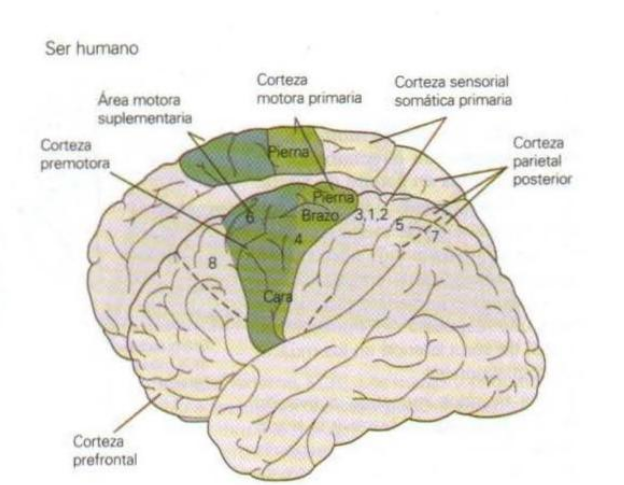
\includegraphics[width=0.4\textwidth]{Imagenes/CortezaMotora.png}
    \caption{Descripción de la imagen.}
\end{figure}

\vspace{1cm}

\subsubsection{EEG}

\subsection{Estado del arte}
Este dataset fue publicado por un conjunto de investigadores de la Universidad Khalifa en Emiratos Árabes Unidos en el artículo \textit{"A Multimodal Gait Dataset of Brain Activity, Muscle Activity, Kinematics and Ground Forces in Young Adults"}. Estos investigadores notaron la necesidad de contar con datasets multimodales que integren la actividad neuronal, muscular, cinemática y cinética de forma sincronizada, ya que estos conjuntos de datos proveen una gran representación de la locomoción humana y resultan útiles para validar modelos computacionales de la marcha y desarrollar algoritmos de \textit{machine learning}.

Para la creación de este dataset, se obtuvieron registros sincronizados de 59 pacientes sanos de $24 \pm 5$ años, de ambos sexos y con diferentes Índices de Masa Corporal. A estos jóvenes adultos se les solicitó caminar en una cinta a distintas velocidades (0.5, 0.75 y 1.0 m/s) con un minuto de recolección de datos por prueba. El \textit{setup} experimental incluía 19 canales de EEG muestreados a 300 Hz utilizando sistemas de electrodos secos bajo el estándar internacional 10-20, 12 sensores de EMG en los principales músculos del tren inferior (usando el sistema Delsys Trigno Wireless EMG), 17 sensores IMU ($fs = 60$ Hz) y una plataforma de fuerza bilateral.

\begin{figure}[h]
    \centering
    
    % --- Primera imagen (Izquierda) ---
    \begin{subfigure}{0.45\textwidth}
        \centering
        % \linewidth hace que la imagen ocupe el ancho disponible de la subfigura
        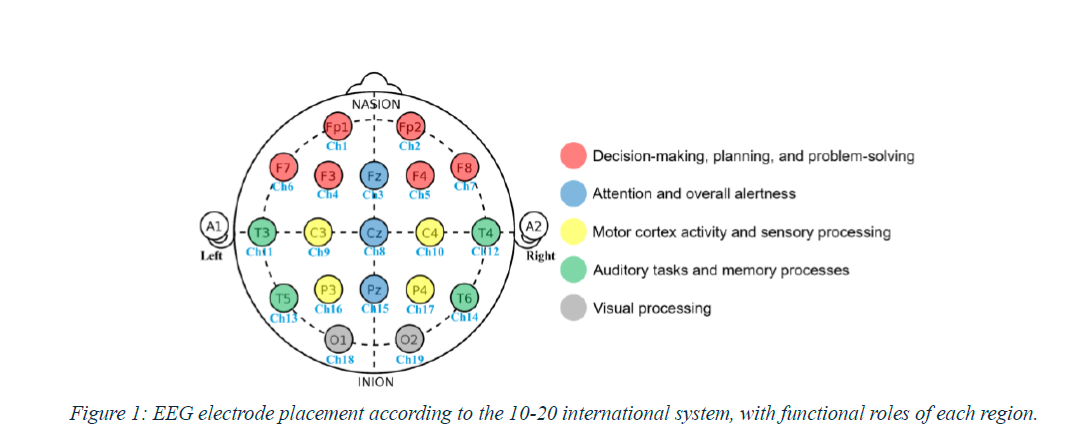
\includegraphics[width=\linewidth]{Imagenes/Sistema 10-20.png}
        \caption{Descripción de la imagen A}
        \label{fig:subim1}
    \end{subfigure}\hfill % El \hfill empuja las imágenes hacia los costados
    % --- Segunda imagen (Derecha) ---
    \begin{subfigure}{0.45\textwidth}
        \centering
        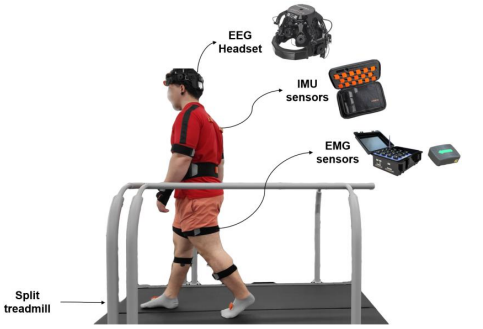
\includegraphics[width=\linewidth]{Imagenes/Setup.png}
        \caption{Descripción de la imagen B}
        \label{fig:subim2}
    \end{subfigure}
    
    \caption{Título general que describe lo que se ve en ambas imágenes en conjunto.}
    \label{fig:imagenes_juntas}
\end{figure}

Como se observa en esta imagen obtenida del artículo original del dataset, las mediciones relacionadas con la actividad motora se concentran en las regiones C3, C4, P3 y P4. Estos electrodos son los que captan la actividad neuronal de las áreas de interés mencionadas en el marco teórico. Por ello, el análisis de este trabajo hará principal foco en dichos canales.


Por otro lado, otra investigación fundamental para el desarrollo de este trabajo práctico fue la publicada en el artículo \textit{"Walking naturally after spinal cord injury using a brain–spine interface"}. Cabe destacar que los integrantes de este grupo de trabajo realizaron previamente una monografía para la materia "16.03 - Fisiología" basada en esta investigación. En síntesis, el estudio detalla la captación de señales electrocorticográficas (ECoG) mediante electrodos implantados, seguido de un procesamiento con modelos de \textit{machine learning} para enviar información a un arreglo implantado de 16 electrodos que produce estimulación medular y genera el movimiento.

En dicho artículo se menciona que, dependiendo de las bandas de frecuencia, es posible identificar el tipo de procesamiento neuronal de la persona. Las ondas Beta (13-30 Hz) determinan la desinhibición y la preparación del movimiento; las ondas Gamma (30-200 Hz) generan la ejecución del movimiento y la coordinación fina; y por último, las ondas Alpha (8-12 Hz) se suprimen cuando existe intención de moverse. A partir del procesamiento de todas estas señales, es factible predecir la intención del paciente, dado que la corteza motora primaria es la encargada de iniciar los procesos de contracción voluntaria. Estos conceptos configuran y respaldan el objetivo central del presente trabajo práctico.
\vspace{1cm}

Por ahi meter alguno más.

https://www.frontiersin.org/journals/human-neuroscience/articles/10.3389/fnhum.2014.00485/full

MuY BUENO ESTE, HAY QUE AGREGARLO


\subsection{Objetivos}

El objetivo general es desarrollar e implementar un algoritmo computacional capaz de procesar señales electroencefalográficas (EEG) para decodificar, analizar y clasificar de manera precisa las distintas fases del ciclo de la marcha humana a partir de la actividad cortical. Los objetivos específicos son:
\begin{itemize}
    \item Diseñar una arquitectura de procesamiento de señales que permita extraer las características espectrales y temporales relevantes del EEG asociadas a la intención motora y la locomoción.
    \item Integrar los parámetros de clasificación obtenidos con el entorno de OpenSim, con el fin de generar una representación visual y cinemática precisa de la marcha basada en el análisis cerebra
    \item Procesar y utilizar los registros multimodales de electromiografía de superficie de los miembros inferiores como método de validación objetiva.
\end{itemize}

Si se realiza una proyección a futuro, se busca un modelo computacionales para el desarrollo de interfaces cerebro-máquina (BCI) no invasivas orientadas a la neurorrehabilitación motora. De manera hipotética, al lograr una decodificación robusta de los correlatos electroencefalográficos vinculados al proceso de marcha, este algoritmo podría integrarse como el núcleo lógico en el sistema de control de exoesqueletos robóticos.

\section{Materiales y Métodos}
\subsection{OpenSIM}

OpenSim es un entorno de software de código abierto desarrollado por el Centro Nacional de Simulación Basada en Física de Estructuras Biológicas de la Universidad de Stanford. Su arquitectura permite desarrollar modelos tridimensionales de alta fidelidad fisiológica y analizar las fuerzas subyacentes que generan el movimiento


El núcleo de OpenSim está construido sobre una serie de herramientas de cálculo computacional avanzado. Entre sus funciones principales se destacan la cinemática inversa, que permite calcular los ángulos articulares óptimos; la dinámica inversa, utilizada para determinar los torques articulares netos; y la optimización estática, que resuelve el problema de la redundancia muscular al estimar las fuerzas musculares individuales. Asimismo, la plataforma permite realizar simulaciones dinámicas, donde un modelo es impulsado por señales de excitación muscular para predecir la cinemática resultante.


Una de las grandes ventajas de OpenSim es su capacidad de integración con lenguajes de programación de alto nivel a través de su API. Esta característica resulta fundamental para el desarrollo de pipelines de procesamiento de señales automatizados.


La integración de OpenSim en el flujo de trabajo computacional permite traducir los resultados de la detección de las fases de la marcha (apoyo y balanceo) en parámetros cinemáticos tangibles. Al visualizar la simulación de la marcha en el modelo musculoesquelético, es posible contrastar las predicciones del modelo neuronal (EEG) con los datos experimentales reales obtenidos mediante electromiografía de superficie (sEMG) y cinemática (IMU). 


\section{Resultados}

\section{Conclusiones}


\section{Bibliografía}

\begin{itemize}
    \item Katmah, R., AlShehhi, A., Kosaji, D., Al-Rahmani, N., Abdullah, M., Hulleck, A. A., \& Khalaf, K. (s.f.). \textit{A Multimodal Gait Dataset of Brain Activity, Muscle Activity, Kinematics and Ground Forces in Young Adults}. Department of Biomedical Engineering \& Biotechnology, Khalifa University.
    \item Lorach, H., Galvez, A., Spagnolo, V., Martel, F., Karakas, S., Intering, N., Vat, M., Faivre, O., Harte, C., Komi, S., Ravier, J., Collin, T., Coquoz, L., Sakr, I., Baaklini, E., Hernandez-Charpak, S. D., Dumont, G., Buschman, R., Buse, N., \dots\ Courtine, G. (2023). Walking naturally after spinal cord injury using a brain--spine interface. \textit{Nature}, \textit{618}(7963), 126--133. https://doi.org/10.1038/s41586-023-06094-5
    \item Kandel, E. R., Schwartz, J. H., \& Jessell, T. M. (2001). Principios de neurociencia (4.ª ed.). McGraw-Hill Interamericana. https://archive.org/details/kandel-e.-r.-j.-h.-schwartz-y-t.-m.-jessell.-principios-de-neurociencia
\end{itemize}



\section{Anexo}





\end{document}
